\documentclass[30pt]{beamer}
\usepackage{graphicx}
%\usetheme{Amsterdam}
\author{ Hsuan-Wei Lee,
  Anzhelika Lyubenko,
  Yuhang Ma,
  Emily Meissen,
  Daniela Velez-Rendon,
    Nara Yoon}


%\vspace{.1truein}

%\begin{center}
%Mentors: John Peach \footnote{Massachusetts Institute of Technology: Lincoln Laboratory}, Cammey Cole Manning\footnote{Mathematics and Computer Science Department, Meredith College},
%Christian Gunning\footnote{Departments of Entomology and Mathematics, North Carolina State University}
%\end{center}
\title[]{Wine, Ebola and Terrorism}

%\date{February 28, 2015}

\begin{document}

\begin{frame}[t,plain]
    \titlepage
\end{frame}

\begin{frame}[t,plain]
    \frametitle{Overview}
\begin{enumerate}
\vfill
\item Introduction
\item Models
\begin{itemize}
\item System-based model
\item Agent-based model
\item Sparial agent-based model
\end{itemize}
\item Comparison
\item Summary
\end{enumerate}
\end{frame}

\begin{frame}
\frametitle{Introduction}
\begin{itemize}
\item Ebola was discovered in 1976
\item 
\end{itemize}
\end{frame}

\begin{frame}
\frametitle{Model}

\begin{figure}[!h]
  \centering
  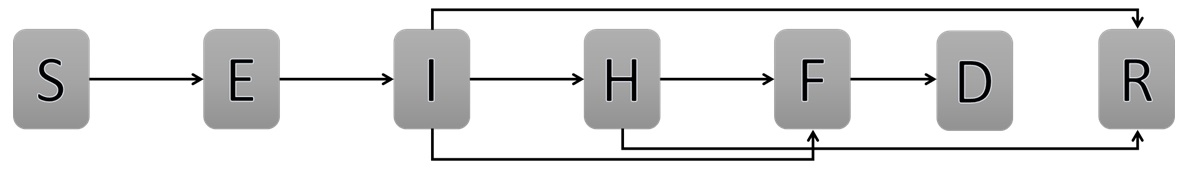
\includegraphics[width=0.7\textwidth]{compartmentNoFlow}
  \caption{Compartment Model of the Ebola Epidemic in Liberia \newline  Being S: Susceptible, E: Exposed, I: Infectious, H: Hospitalized, F: Funeral,  R: Recovered and D: Dead. All the possible flows are specified by the arrows and the parameters that direct them. Note that $\lambda = \beta_{I}I+\beta_{H}H+\beta_{F}F $, is a combination of all the $\beta$ transmission terms shown in Table~\ref{tab:parameters} } 
\label{fig:compartment} 
\end{figure}
\end{frame}

\begin{frame}
\frametitle{Assumptions}
\end{frame}

\begin{frame}
\frametitle{Parameters/Data}
\begin{figure}[!h]
  \centering
  \includegraphics[width=0.7\textwidth]{tab_para}
  \caption{Model Parameters for Ebola Epidemic in Liberia Before and After the International Intervention. Calibrated parameters are written in bold font, and posterior means and standard deviations in parenthesis are notated. } 
\label{fig:compartment} 
\end{figure}

\end{frame}

\begin{frame}
\frametitle{System model}
\end{frame}

\begin{frame}
\frametitle{System Model Results}
\end{frame}

\begin{frame}
\frametitle{Agent model}
\end{frame}

\begin{frame}
\frametitle{Agent Model Results}
\end{frame}

\begin{frame}
\frametitle{Spatial Agent Model}
\end{frame}


\begin{frame}
\frametitle{Spatial Agent Model Results}
\end{frame}

\begin{frame}
\frametitle{Comparison}
\end{frame}

\begin{frame}
\frametitle{Summary}
\end{frame}
\end{document}